\documentclass[12pt]{article}
	
\usepackage[margin=1in]{geometry}		% For setting margins
\usepackage{amsmath}				% For Math
\usepackage{amssymb} % For \mathbb
\usepackage{fancyhdr}				% For fancy header/footer
\usepackage{graphicx}	% For including figure/image
\renewcommand{\contentsname}{Table of Contents}
\usepackage{enumitem}
\usepackage{cancel}					% To use the slash to cancel out stuff in work
\usepackage[margin=0.25in]{geometry}
\usepackage{hyperref}
\usepackage{float}
\usepackage{indentfirst}
\usepackage[american, siunitx]{circuitikz}
\usepackage{circuitikz}
\usepackage{lipsum}
\usepackage{setspace}
\usepackage{fontspec}
\setmainfont{Times New Roman}



\pagestyle{fancy}
\fancyhead[LO,L]{Mark Le}
\fancyhead[CO,C]{}
\fancyhead[RO,R]{\textbf{ELECENG 2EI4 Project 1 - AC to DC Converter}}
\fancyfoot[LO,L]{}
\fancyfoot[CO,C]{\textbf{\thepage}}
\fancyfoot[RO,R]{}


%%%%%%%%%%%%%%%%%%%%%%

\spacing{1.25}
\begin{document}
    
    \begin{titlepage}
    \begin{center}
    \vspace*{\fill}

    {\LARGE \textbf{ELECENG 2EI4 - Electronic Devices \& Circuits I}\par}
    \vspace{2.5cm}

    {\LARGE\bfseries Project 1 - AC to DC Converter\par}
    \vspace{2.5cm}
    
    {\Large \textbf{Mark Le - 400558145}\par}
    \vspace{2.5cm}
    
    {\large Instructor: Dr. Yaser M. Haddara\par}
    \vspace{0.5cm}
    {\large Term: Winter 2026 \par}
    \vspace{0.5cm}
    
    {\large \textbf{Submission Deadline:} Sunday, February 8, 2026\par}
    \end{center}

    \vspace*{\fill}

    \textbf{Statement of Originality:} As a future member of the engineering profession, the student is responsible for performing the required work in an honest manner, without plagiarism and cheating. Submitting this work with my name and student number is a statement and understanding that this work is my own and adheres to the Academic Integrity Policy of McMaster University and the Code of Conduct of the Professional Engineers of Ontario. Submitted by \textbf{Mark Le, lek37, 400558145}

\end{titlepage}

    \newpage
    \tableofcontents

    \listoffigures

    \listoftables

    \newpage
    \section{Summary}

    The purpose of this project is to convert the AC 120 V RMS signal to a 3.0 V \(\pm\) 0.1 V DC output signal. This design can be achieved by implementing a transformer, a rectifier, a filter and a regulator. A transformer is theoretically implemented to lowered the AC RMS voltage to a desired value, a rectifier transforms the negative half cycle to positive, create a DC signal, a capacitor is used as a filter to generate a smooth ripple. Additionally, a resistor acts as a load to measure the output DC voltage.  
    
    \section{Design}
    DC power supply design elements descriptions:
    \begin{itemize}
        \item Transformer: through the calculation, the input voltages required for my design was found to be 5.4 V RMS, where each half of the diode will be supplied approximately 2.7 V RMS, at 1 kHz. The primary voltage is defined to be \(V_p=120 V\) RMS, and the secondary voltage is defined to be \(V_s=5.4V\) RMS, therefore the turn ratio is:
        \begin{equation}
            \frac{V_p}{V_s}=\frac{N_p}{N_s}=\frac{120}{5.4} \approx 22.2
        \end{equation}
        Thus, we need a 120 V:5.4 V step-down transformer, in which the turns ratio is approximately 22:1. 

        \item Rectifier: for this design, I used a full-wave center-tapped rectifier, with the topology shown below:

        \begin{figure}[H]
            \centering
            \caption{Full-wave center-tapped rectifier topology}
            \vspace{0.3cm}
            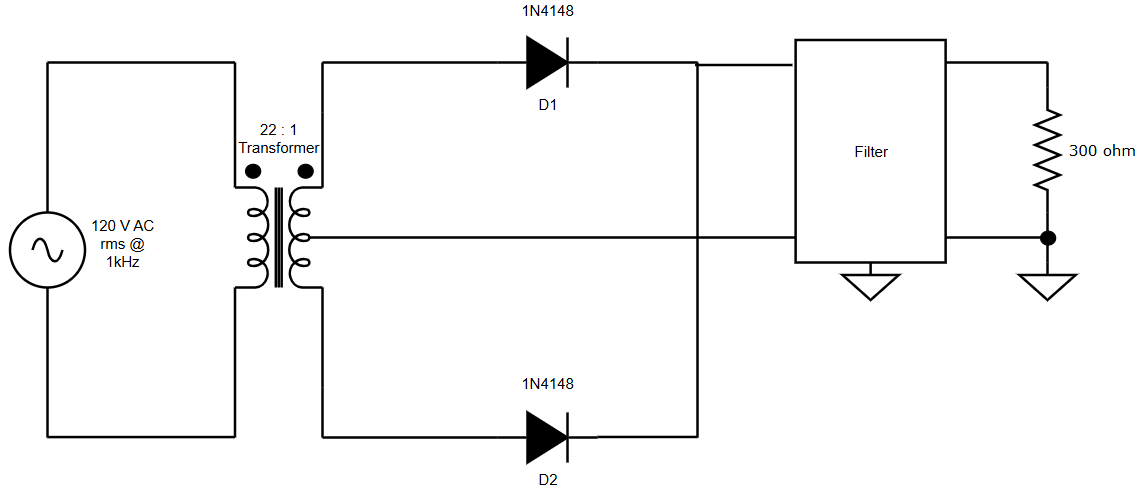
\includegraphics[width=1\linewidth]{Screenshot 2026-02-07 150220.png}
        \end{figure}

            
            Justifications: the reason why I chose this rectifier topology is because it can convert the AC signal to DC by "flipping" the negative half-wave input into a positive, DC input effectively. In particular, this rectifier configuration produces lower voltage ripple compares to the half-wave rectifier, due to higher frequency rectified. Additionally, while experimenting with the full wave bridge rectifier, the voltage output deviated significantly compared to the full-wave center-tapped rectifier, since less diodes are being used. The diode 1N4148 parameters are:
            
        \begin{itemize}
            \item Forward-bias voltage: \(V_D=0.7V\) [2]
            \item Breakdown voltage: 75-100 V [2]
        \end{itemize}

        \item Filter: I used a capacitor CM107M (came from 2CI4 kit) as a filter, has a capacitance of 100 \(\mu\)F.
        
        \item Regulator: none
        \item Complete circuit schematics:

        \begin{figure}[H]
            \centering
            \caption{Full circuit schematic}
            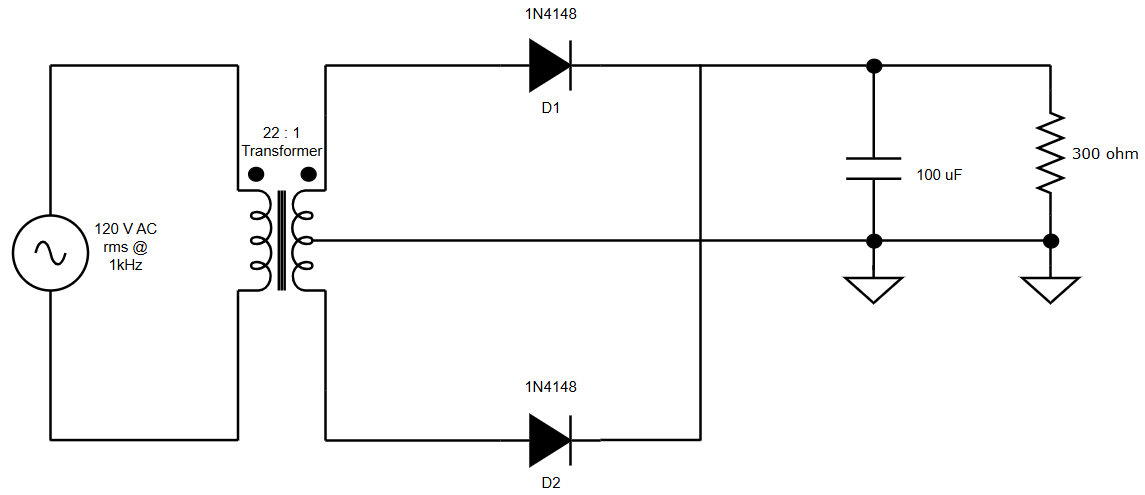
\includegraphics[width=1\linewidth]{Screenshot 2026-02-07 010234.png}
        \end{figure}


        \item Calculations: for the load resistor \(R_L\), we know that the output voltage must be 3 V (\(\pm\) 0.1 V), and it must has a current of 10 mA goes through it, therefore:
        \begin{equation}
            R_L=\frac{V_{o}}{I_{o}}=\frac{3V}{10mA}=300 \Omega
        \end{equation}

        \textit{This calculation is based on the theoretical expected output voltage and current, in which \(V_0=3.0V\) and \(I_0=10mA\)}

        Since the full-wave rectifier invert the negative half-wave cycle, the ripple frequency \(f_{rpp}\) becomes doubled, that is:
        \begin{equation}
            f_{rpp}=2f_{in}=2(1kHz)=2kHz
        \end{equation}

        We are given the formula for finding the ripple voltage; it is inversely proportional to the capacitor. Since the design requirement wants the ripple voltage to be \(\pm\) 0.1 V, \(V_{rpp}=0.2V\). Therefore:
        \begin{equation} V_{rpp}=\frac{I_{o}}{f_{rpp}C} \Rightarrow C=\frac{I_o}{V_{rpp}f_{rpp}}=\frac{10mA}{(0.2V)(2kHz)}=25 \mu F
        \end{equation}

        This is the minimum capacitance needed to produce a 0.2 V ripple. So I chose the 100 \(\mu\)F capacitor in the 2CI4 kit. 

        For finding the required AC voltage into the rectifier, we must found the minimum allowable input AC peak voltage into the rectifier. Since the expected output is 3.0 \(\pm\) 0.1V, the ripple voltage is 0.2 V. Denote the peak AC input voltage as \(V_{AC,peak}\), and the maximum capacitor voltage being \(V_{C,max}\). It is known that:
        \begin{equation}
            V_{C,max}=V_{AC,peak}-V_D 
        \end{equation}
        \begin{equation}
            V_{C,max}=V_{AC,peak}-0.7V
        \end{equation}
        On the other hand, the DC output voltage is defined to be:
        \begin{equation}
            V_{DC}=V_{C,max}-\frac{V_{rpp}}{2}
        \end{equation}
        By substitute (5) into (6), we obtain:
        \begin{equation}
            V_{DC}=V_{AC,peak}-\frac{V_{rpp}}{2}-0.7V
        \end{equation}
        \begin{equation}
            V_{AC,peak}=V_{DC}+\frac{V_{rpp}}{2}+0.7V
        \end{equation}
        \begin{equation}
            V_{AC,peak}=3.0V+0.1V+0.7V=3.8V
        \end{equation}

        To find RMS value:
        \begin{equation}
            V_{AC,RMS}=\frac{V_{AC,peak}}{\sqrt{2}}=\frac{3.8V}{\sqrt{2}}=2.7 V
        \end{equation}
        which give a total of 5.4 V RMS as a secondary voltage of the transformer. Therefore, we need two waveforms as a voltage supply to the rectifier:
        \begin{itemize}
            \item To diode D1: \(\tilde{\mathbf{V}}_{D1} = 3.8 \angle 90^\circ\) (V)
            \item To diode D2: \(\tilde{\mathbf{V}}_{D2} = 3.8 \angle {-90^\circ}\) (V) \(\to\) \textit{must be out of phase \(180^0\) with respect to \(\tilde{\mathbf{V}}_{D1}\)}
        \end{itemize}

        \item Expected performance: as discussed, there should be only one diode forward-biased at a time, which produced a voltage drop of 0.7 V. Addtionally, since a 100 \(\mu\)F capacitor is used, the expected ripple voltage would be:
        \begin{equation}
            V_{rpp}=\frac{I_0}{f_{rpp}C}=\frac{10mA}{(2kHz)(100\mu F)}=0.05 V
        \end{equation}

        Therefore the expected output voltage is \(V_0=3.0V \pm 0.025V\)

        \item Design safety consideration: 


        For the resistors: Since I don't have a single 300 \(\Omega\) resistor, I use a combination of two 150 \(\Omega\) resistors instead. Each resistor has a tolerance of \(\pm\)5\%, so the maximum resistance for each is 157.5 \(\Omega\) These resistors have a power rating of 0.25 W (R 1/4). Since each 150 \(\Omega\) resistor carries a current of 10 mA, we have:
        \begin{equation}
            P_{150\Omega,max}=I^2R=(0.01A)^2(157.5 \Omega)=0.016W <0.25W
        \end{equation}
        Thus, the resistors are safety implemented. 

        For the capacitor: we must verify that the voltage rating check cannot exceed 6.3 V. The rectifier input peak is 3.8 V, as proven above. After finish charging, the capacitor acts as a voltage source, and the voltage across it is dropped by 0.7 V due to the current goes through one diode at a time. Therefore the voltage across the capacitor when finish charging is:
        \begin{equation}
            V_{C,max}=V_{peak}-V_D=3.8V-0.7V=3.1V<6.3V
        \end{equation}

        Thus, the capacitor is safely implemented.  

        For the diodes: according to the datasheet from \textit{Abra Electronics}, the maximum reverse voltage is about 100 V [4]. In the circuit, since the maximum reverse-voltage estimate per diode is approximately 3.8 V, this is still far from the danger zone. The average forward current for this diode is said to be 150 mA, with the repetitive peak forward current up to 500 mA [4], but since only each diodes only conduct a maximum current of 10 mA at a time, it is still in a safety zone. We can also find the power dissipation check on this diode model during conductance zone:
        \begin{equation}
            P_D \approx V_DI=(0.7V)(0.01W)=7mW
        \end{equation}
        And since the limit power dissipation of the 1N4148 diode is 500 mW [4], the design is fully proven to be safety to operate on the AD3.
    \end{itemize} 

    \section{Measurement \& Analysis}
    
    \begin{figure}[H]
        \centering
        \caption{My circuit built on breadboard with name, student number, and date}
        \vspace{0.3cm}
        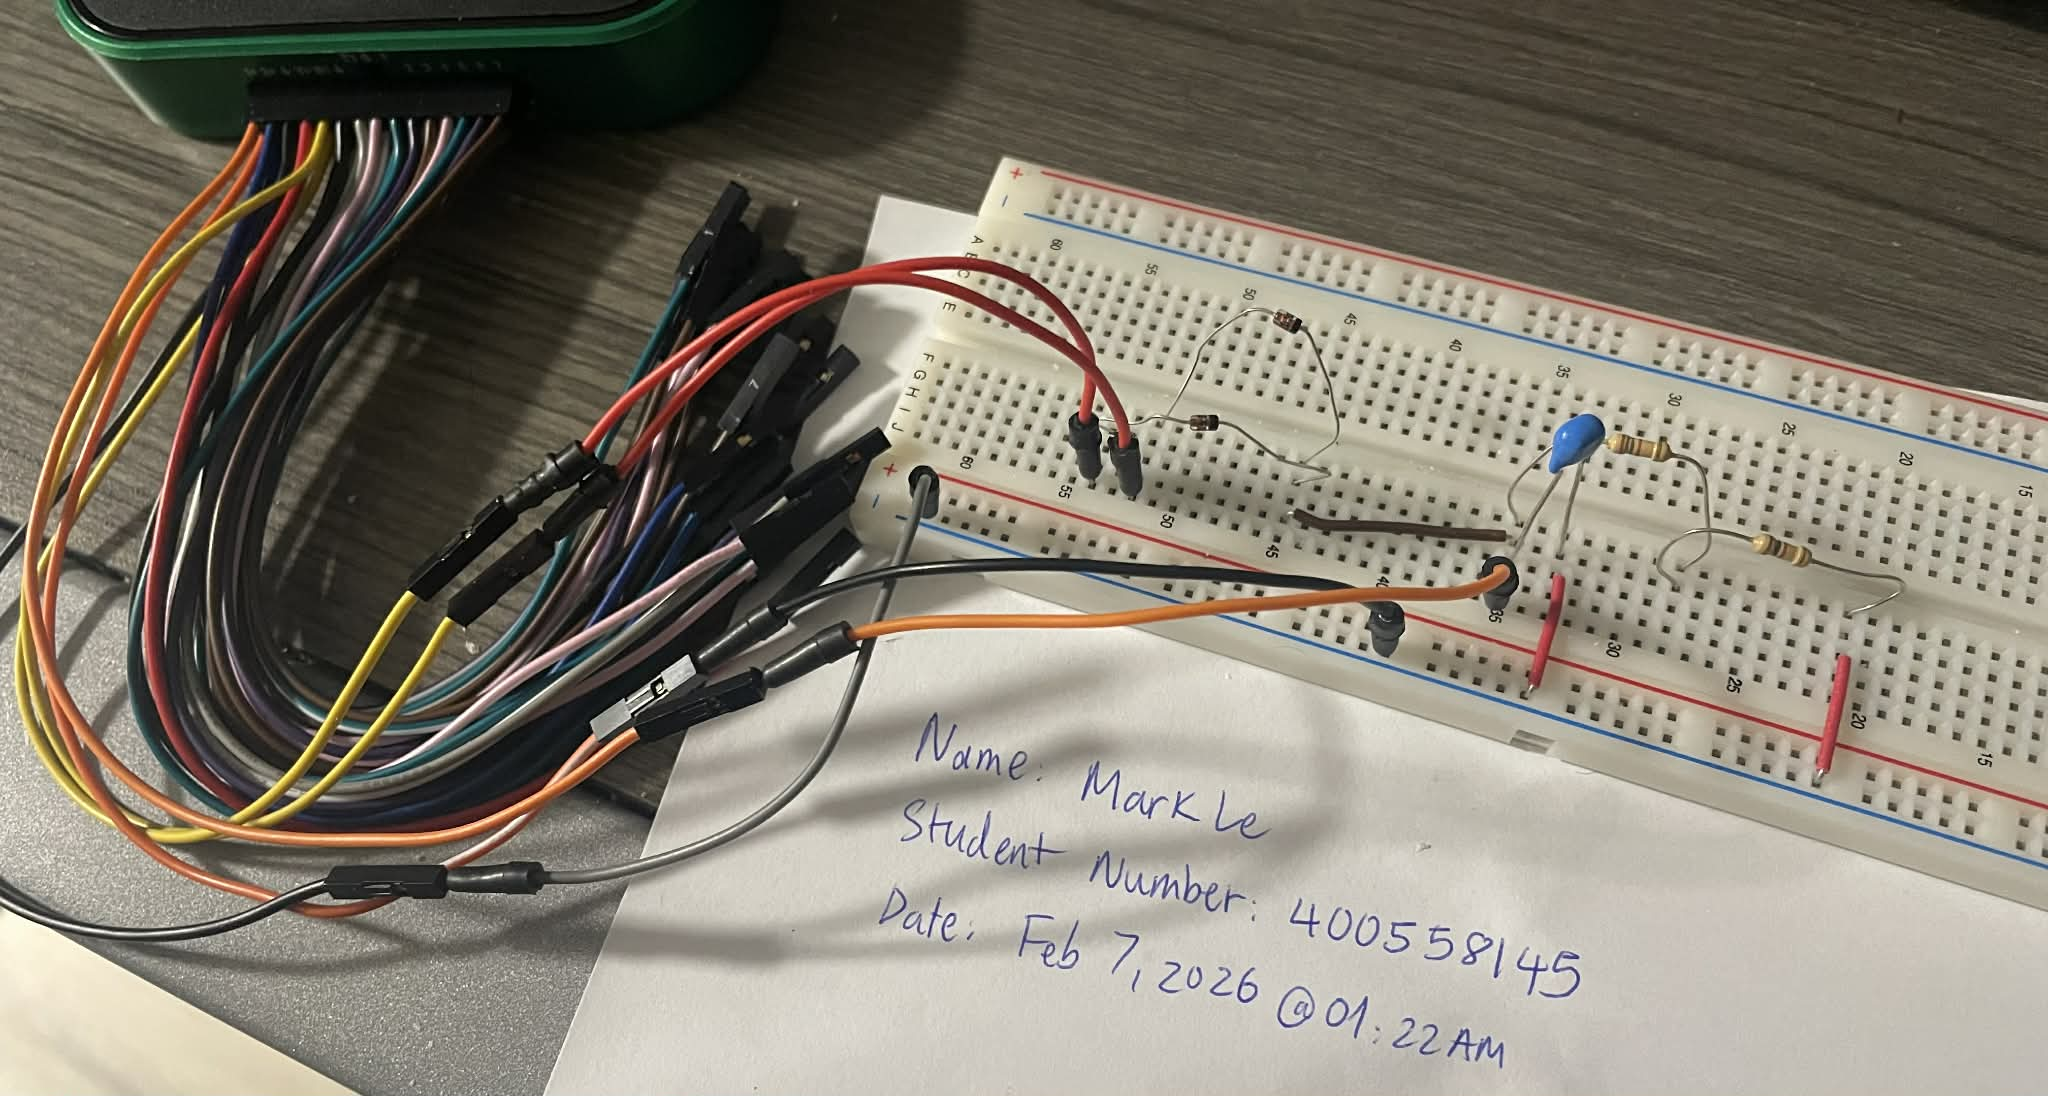
\includegraphics[width=0.8\linewidth]{circuit.jpg}
    \end{figure}

    \begin{itemize}
        \item Measurement procedure: to find the voltage output, I used an Analog Discovery 3 (AD3) to generate a waveform W1, supplying the diode D1 (node 54 on breadboard), and waveform W2, supplying the diode D2 (node 52 on breadboard). Since the AD3 can't find current directly, I took the output voltage measured and divided by 300, according to Ohm's Law. The figure below shows how I set up two wavegens for generating an input signal to the diodes. 

        \begin{figure}[H]
            \centering
            \caption{Wavegen for diodes}
            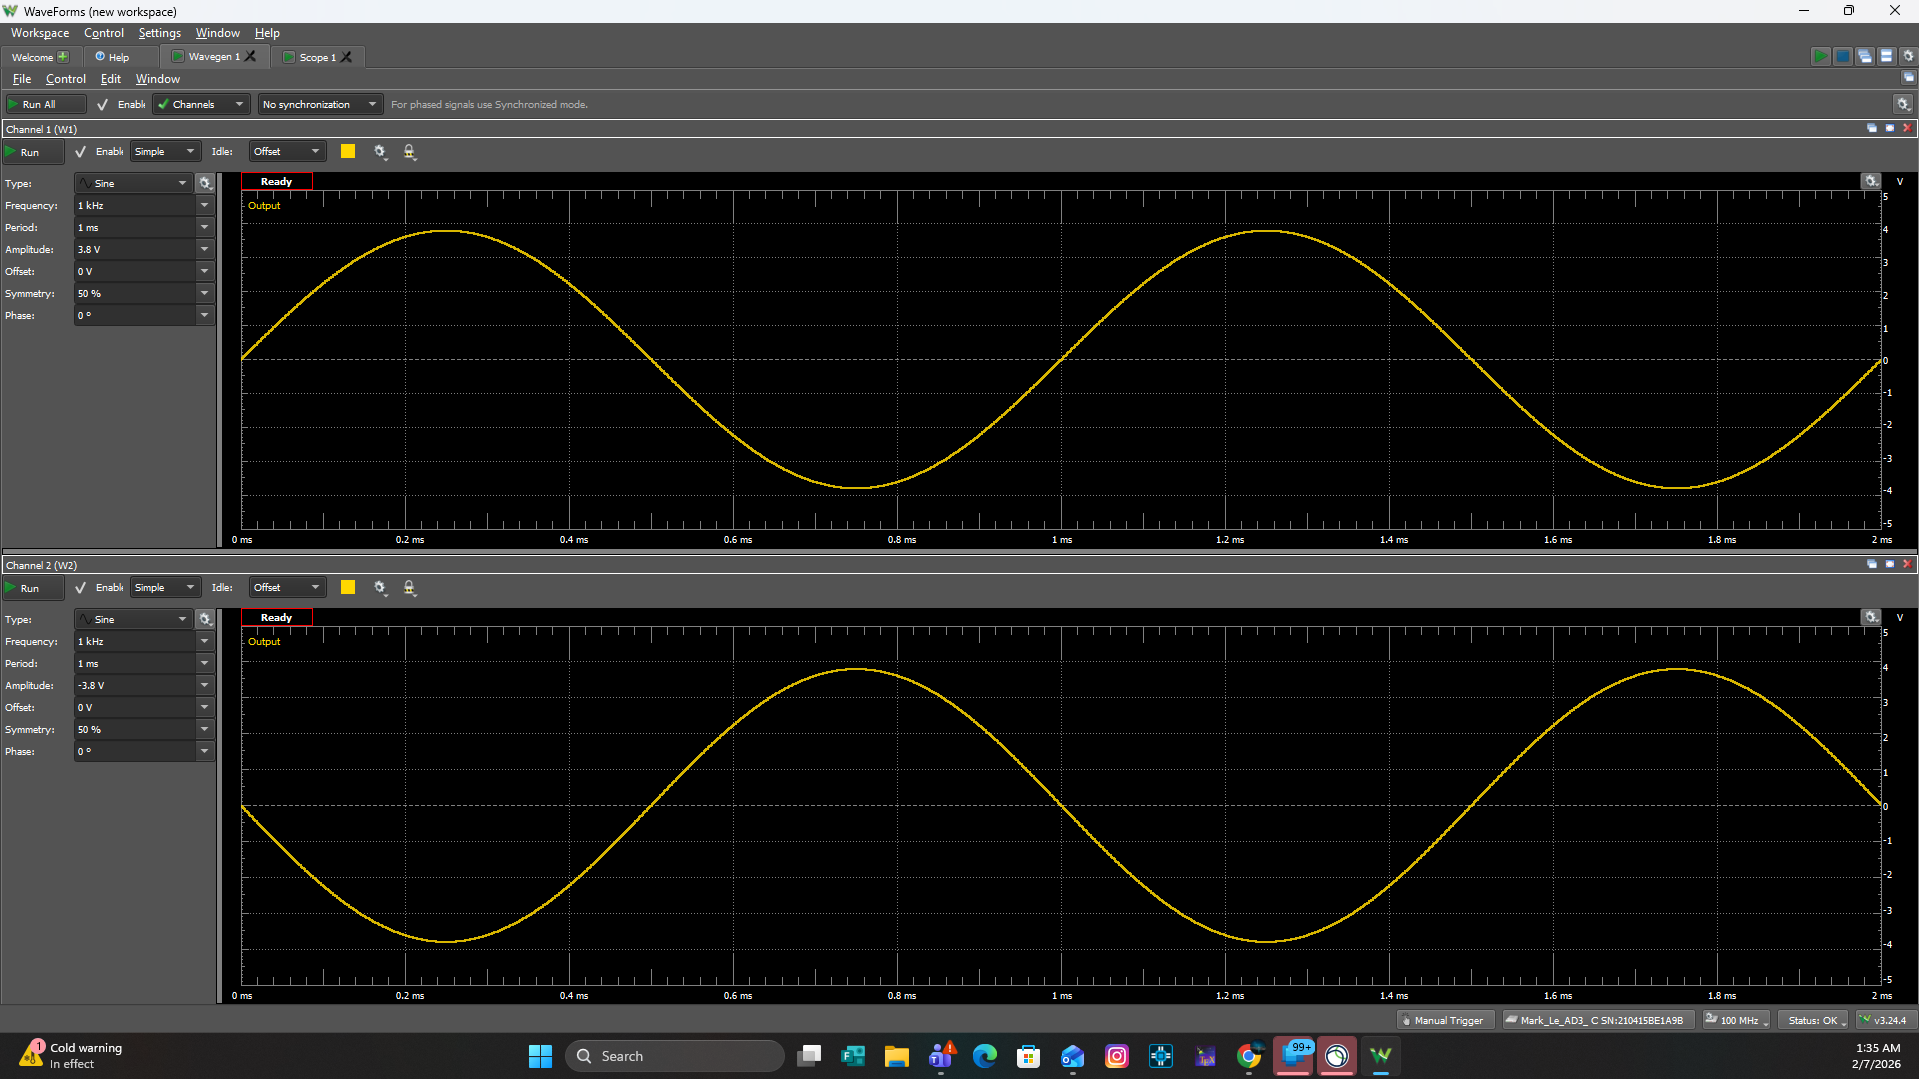
\includegraphics[width=0.8\linewidth]{Screenshot 2026-02-07 013513.png}
        \end{figure}

        \item Measurement results: this is the plot of the output voltage \(V_0\), generated by the AD3 Channel 1:
        \begin{figure}[H]
            \centering
            \caption{Plot of \(V_0\)}
            \vspace{0.3cm}
            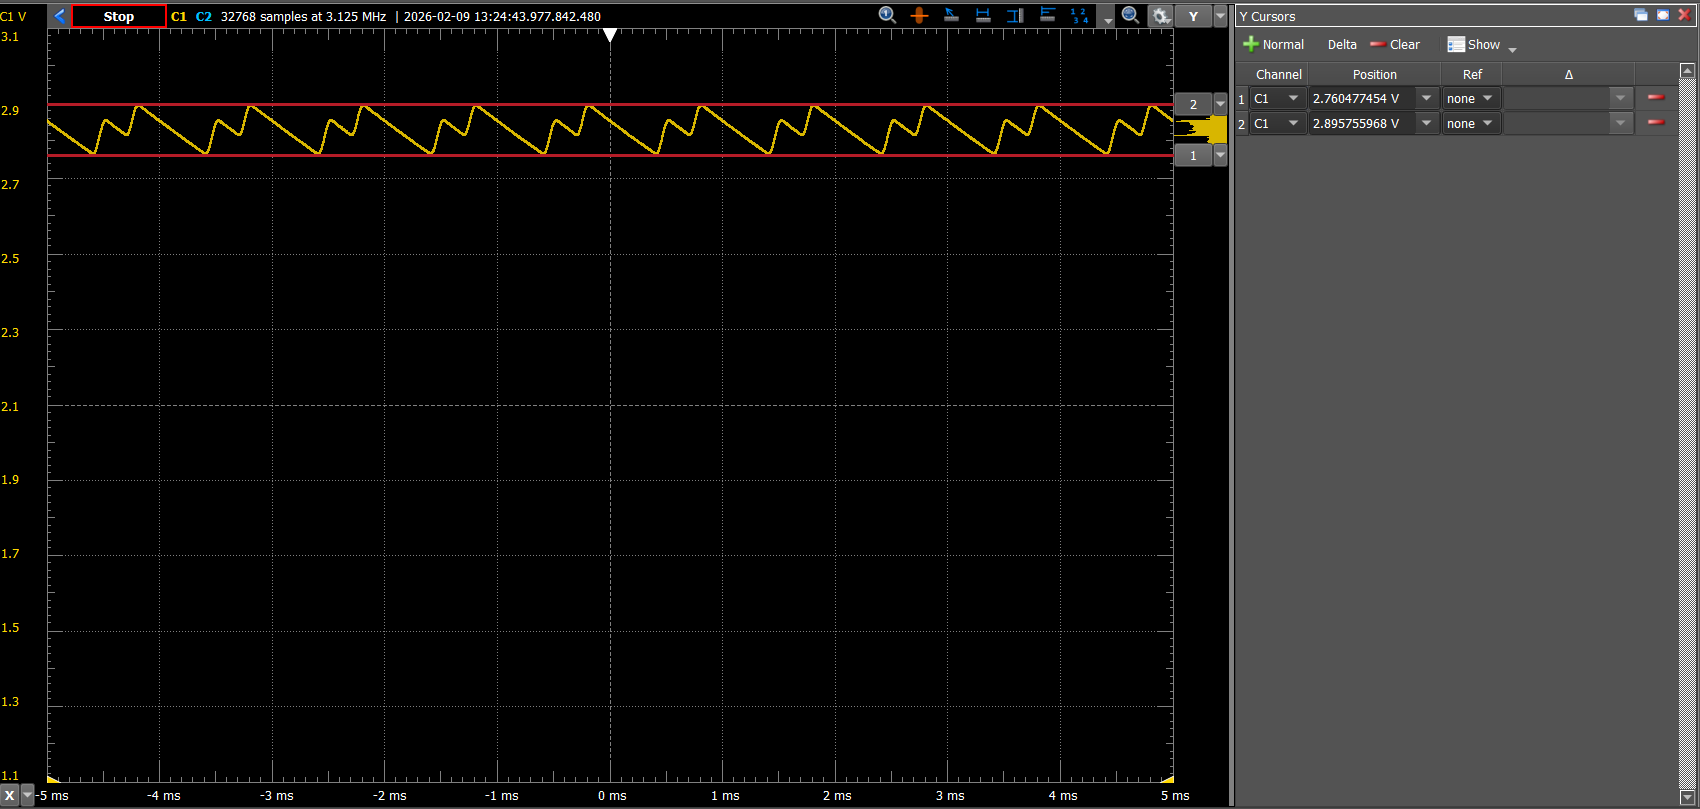
\includegraphics[width=1.0\linewidth]{Screenshot 2026-02-09 132624.png}
        \end{figure}
    \end{itemize}


    \textbf{Observation:} it is obvious that the experimental result of \(V_0\) deviates a bit from our expectation. It is expected that the output voltage should be in the range of [2.975, 3.025] V, as the design expected. However, the plot shows that the output fluctuates between 2.76 V and 2.90 V, which leds to the output current being around 9.30 to 9.67 mA.

    \newpage
    \section{Simulation}
    This my LTspice of the circuit implementation, for a purpose of simulation
    \begin{figure}[H]
        \centering
        \caption{LTspice schematic of my circuit}
        \vspace{0.3cm}
        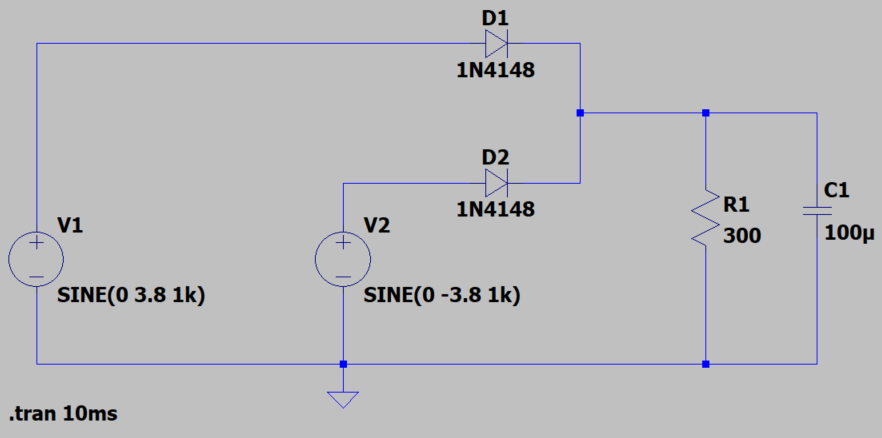
\includegraphics[width=0.9\linewidth]{Screenshot 2026-02-07 024216.png}
    \end{figure}

    As for supplying the input AC voltage for diode D1 and D2 (both are specified by 1N4148 model), I used the sine wave, with the amplitude of 3.8 V, came from the theoretical derivation in equation (10), at 1kHz frequency. Note that for \texttt{V2}, I put the amplitude of -3.8 V, making it \(180^0\) out of phase compared to \texttt{V1}. I used a resistor value of 300 \(\Omega\) and capacitor of 100 \(\mu\)F, as from the theoretical derivation on equation (2) and (4) above. For simulation, I perform a time-domain simulation by specifying a stop time of 10 ms. To measure \(V_0\), I placed the probe on the node between the capacitor (filter) and the resistor (load). This will give a plot of \(V_0\) over time. I also measured the input voltage to the rectifier and put all three plots in the same plot table. The figure below shows the plot:

    \begin{figure}[H]
        \centering
        \caption{LTspice plot of \(V_0\) and \(I_0\)}
        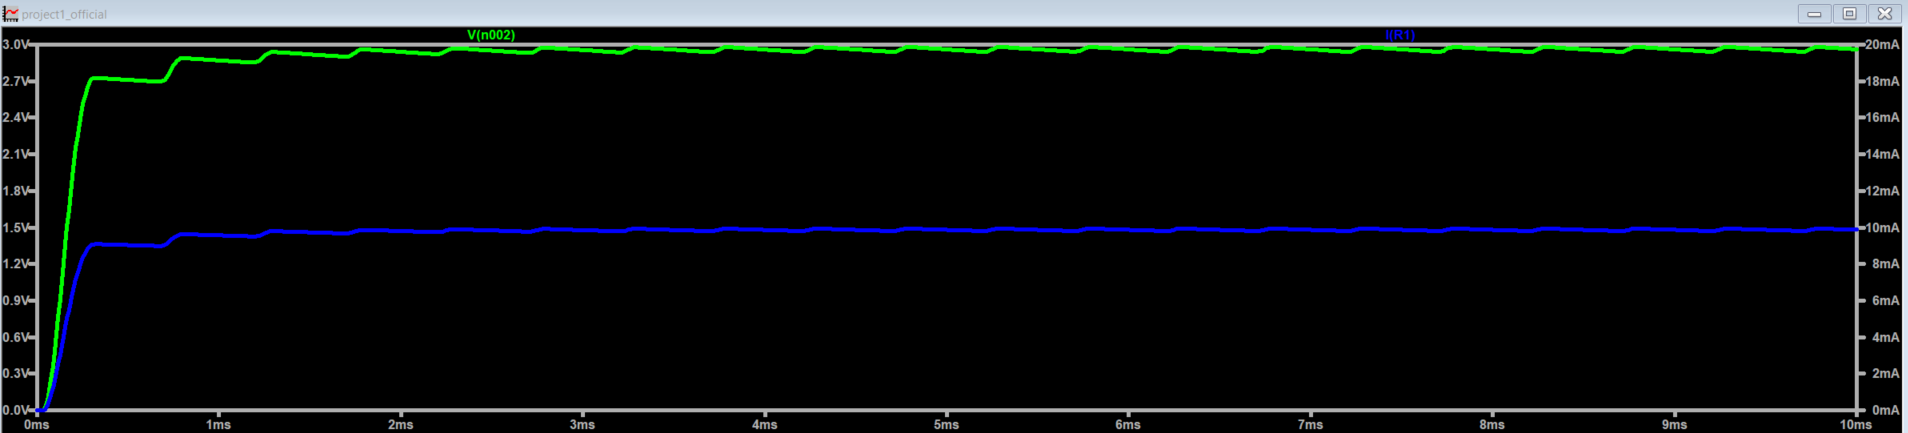
\includegraphics[width=1.1\linewidth]{Screenshot 2026-02-07 025332.png}
    \end{figure}
    
    Netlist:
    \begin{verbatim}
* C:\Users\ankhu\OneDrive\Desktop\ELECENG 2EI4\project1_official.asc
* Generated by LTspice 26.0.1 for Windows.
V1 N001 0 SINE(0 3.8 1k)
V2 N003 0 SINE(0 -3.8 1k)
D1 N001 N002 1N4148
D2 N003 N002 1N4148
R1 N002 0 300
C1 N002 0 100µ
.model D D
.lib C:\Users\ankhu\AppData\Local\LTspice\lib\cmp\standard.dio
.tran 10ms
.backanno
.end
    \end{verbatim}

    \textbf{Observation:} through the LTspice simulation, it is clear that the output (green curve) voltage is fairly consistent with our expectation. It can be seen that the voltage stays in the range of [2.95, 3.0] V, and the output current is shown to be in the range of [9.79, 9.96] mA (blue curve), which is also consistent with our expectation.

    \newpage
    \section{Discussion}

    Through the design, measurement, and simulation, the table below shows the output:

    \begin{table}[H]
        \centering
        \caption{Summary of theoretical (design) and experimental (AD3 \& LTspice) output}
        \vspace{0.3cm}
        \begin{tabular}{|c|p{3.5cm}|p{3.5cm}|p{3.5cm}|}
            \hline
             & \textbf{Design} & \textbf{AD3 Measurement} & \textbf{LTspice Simulation}  \\ \hline
            \textbf{Output DC voltage} \(V_0\) (V) & [2.975, 3.025] & [2.76, 2.90] & [2.95, 3.00] \\ \hline
            \textbf{Output current} \(I_0\) (mA) & [9.92, 10.08] & [9.30, 9.67] & [9.79, 9.96] \\ \hline
        \end{tabular}
    \end{table}

    \textbf{Discrepancies}: it is obvious that the AD3 simulation causes the most significant discrepancies. One possible reason behind this huge discrepancies is because the AD3 results came from the physical circuit with real components. Since the 150 \(\Omega\) resistors have \(\pm\)5\% tolerance rate (the outer band color is gold), the load resistance can ranges from [285, 315] \(\Omega\). Moreover, the diode 1N4148 drop voltage may not exactly 0.7 V all the time. Under certain conditions, this diode can allow a \textbf{maximum} of 1 V of drop down voltage across it. This systematic error leads to incorrect results from the AD3 simulation. Internal circuitry inside the AD3 itself also contribute to the error, since the design does not consider it. As a result, when the peak AC input voltage is adjusted to 4.0 V, the results seems to be more accurate, as it can be seen that the output voltage ranges from [2.88, 3.09] V, which yield an average output voltage of 2.99 V, and the average current of 9.97 mA.  

    \begin{figure}[H]
        \centering
        \caption{Alternate output voltage when \(V_{AC,peak}=4.0V\)}
        \vspace{0.3cm}
        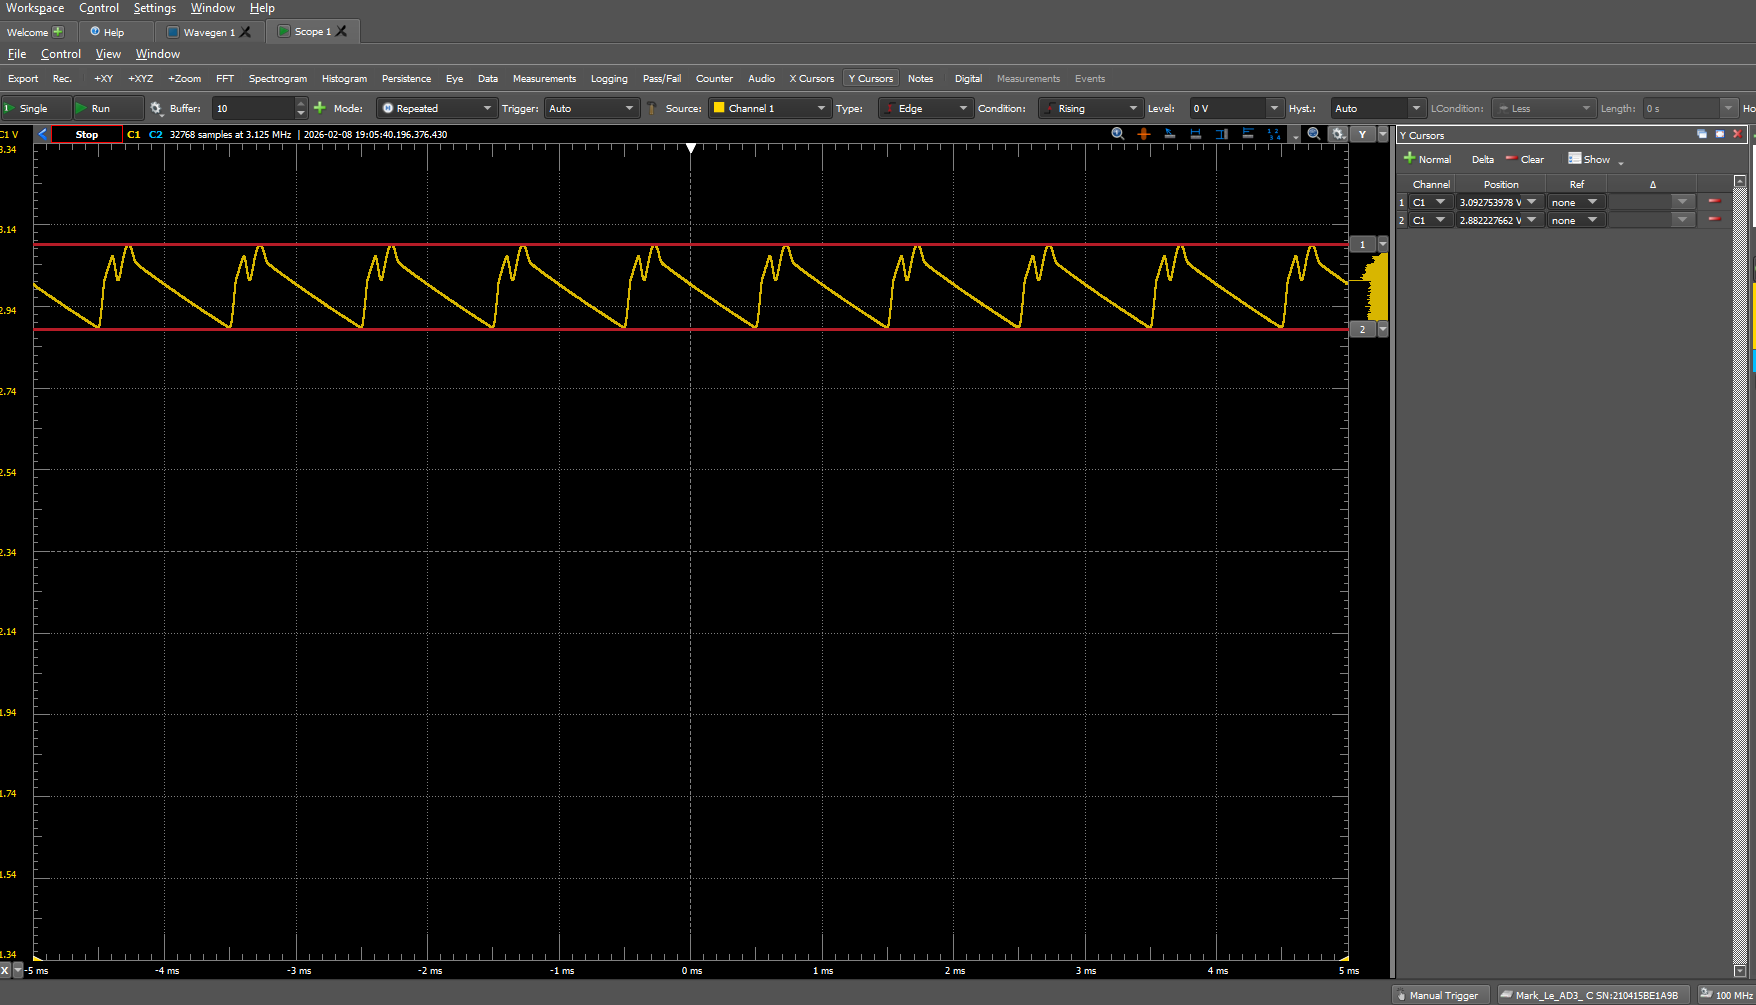
\includegraphics[width=1\linewidth]{Screenshot 2026-02-08 190959.png}
    \end{figure}

    
    As for the LTspice simulation, though the measurement are not completely exact, it can be seen that there are no noticeable discrepancies, as the average output voltage is found to be 2.98 V, and the average current measured is found to be 9.88 mA. A possible reason behind this is LTspice simulation yield theoretical result, which can be more accurate compared to the AD3 simulation. That is, no physical components are involved in the design and simulation process.

    \textbf{Design Limitations:} as for this design project, there are many limitations regarding the design process. As discussed, the resistors used aren't yield exact resistance (tolerance = 5\%), which result in slight deviated measurement in output voltage and current. Additionally, 0.7 V isn't always the voltage drop for the 1N4148 diodes, causing inconsistent results of measuring output voltage and current. The capacitor CM107 also has a tolerance capacitance of 20\%, since it depends on the temperature and frequency of operation. That makes the ripple voltage became inconsistent with the theoretical expectation, and thus affecting the output measurements. 


    \textbf{Troubleshooting:} there were many problem while building the circuit for AD3 simulation. First of all, I connected a wrong terminal of the diode. This result in the voltage measured being around 0 - 0.25 mA (almost result in an open circuit). Additionally, even though the circuit was correctly built, the AD3 simulation deviated from the expected result by a large margin. As a result, I had to keep increasing the amplitude of the AC input voltage until the simulation became close to the desired output. After iterating the peak AC input voltage, \(V_{AC,peak}=4.0V\) yield the most accurate output.  

    \newpage
    \begin{thebibliography}{9}

    \bibitem{CircuitBreadFWCT}
        CircuitBread, ``Center Tapped Full-Wave Rectifier Operation,'' 
        [Online]. Available: https://www.circuitbread.com/tutorials/center-tapped-full-wave-rectifier-operation. Accessed Feb, 7. 2026.

    \bibitem{ONsemiPDF}
        ON Semiconductor, ``1N4148 Switching Diode Datasheet,'' 
        [Online]. Available: https://www.onsemi.com/pdf/datasheet/1n4148-d.pdf. Accessed Feb, 7. 2026

    \bibitem{AbraCap}
    Abra Electronics, ``CM107 Ceramic Capacitor, 100 $\mu$F, 6.3 V, X5R,'' 
    [Online]. Available: https://abra-electronics.com/passive-components/capacitors/ceramic-monolithic-capacitors-radial/cm107-capacitor-ceramic-100uf-20-6-3-volts-x5r-5mm.html. Accessed Feb, 7. 2026

    \bibitem{AbraDiode}
    Abra Electronics, "1N4148 Diode Small Signal Fast Switching 0.3A 100V," [Online]. Available: https://abra-electronics.com/ics-semiconductors/diodes-rectifiers/switching-diodes/1n4148-diode-small-signal-fast-switching-03a-100v-1n4148.html. Accessed Feb, 8. 2026
    \end{thebibliography} 
\end{document}
